\section{Clustered HFL}

Besides classic FL, FLOps supports (clustered) HFL.
Oakestra's three-tiered layout supports geographically dispersed clusters.
Each cluster has its own cluster orchestrator and set of worker nodes.
This structure naturally alludes to the use of clustered and hierarchical FL.
Remembering Figure \ref{fig:uml_project_aggregators_analysis_object_model}, FLOps uses two different types of aggregators for HFL.
The root and cluster aggregators are deployed as services on worker nodes to distribute computational load.
Only a single root aggregator exists.
It can reside in any cluster.
Each orchestrated cluster hosts a single cluster aggregator.
A cluster aggregator only works with learners inside the same cluster.
This type of geographic clustering is why FLOps' HFL is a clustered approach.
Root aggregators treat cluster aggregators as plain learners, precisely as in classic FL.
Cluster aggregators are a combination between learner and aggregator.
Note that Flower does not natively support HFL.
Therefore, this approach of realizing HFL via Flower is a custom novel solution.

\begin{figure}[p]
    \begin{adjustwidth}{-0.1\paperwidth}{-0.1\paperwidth}
        \centering
        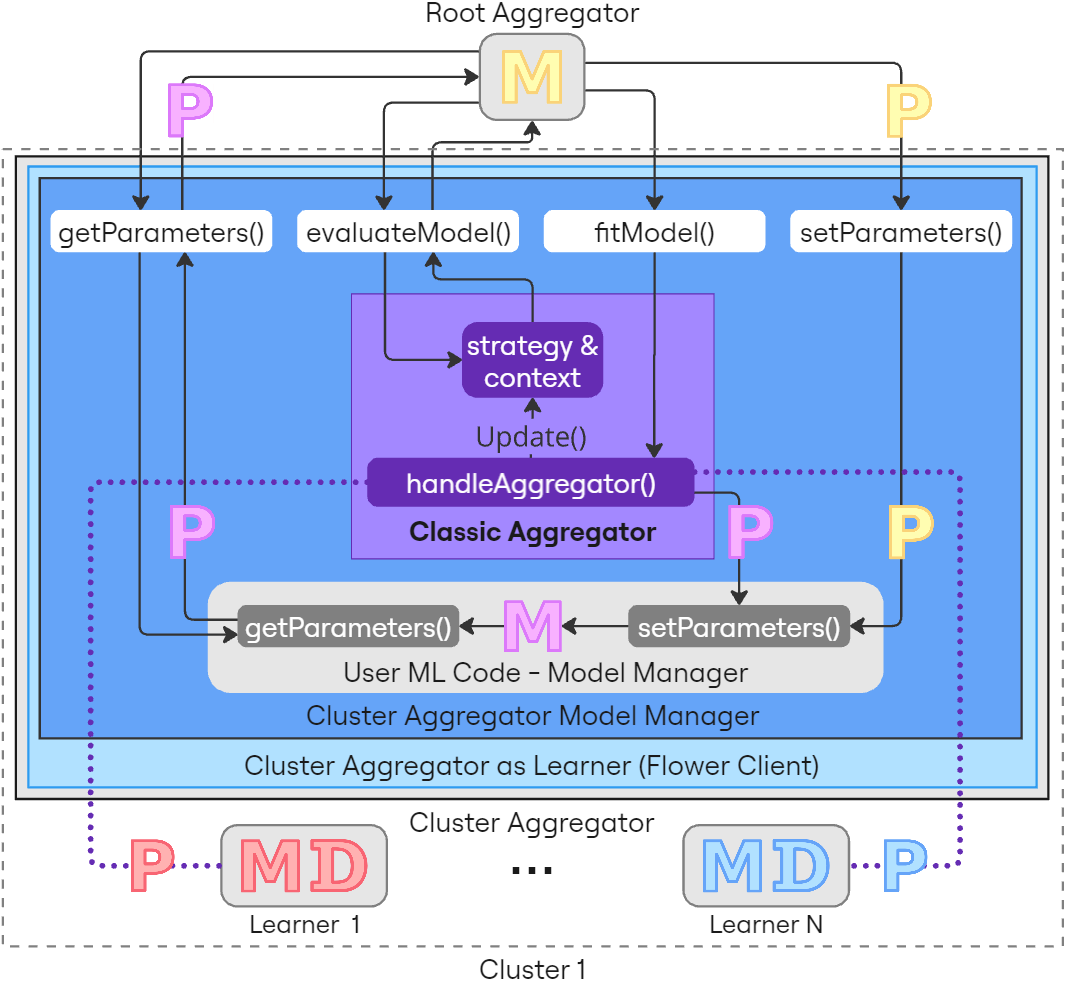
\includegraphics[width=0.80\paperwidth]{clustered_hfl_architecture.png}
        \caption{FLOps clustered HFL Architecture}
        \label{fig:flops_clustered_hfl_architecture}
    \end{adjustwidth}
\end{figure}
Figure \ref{fig:flops_clustered_hfl_architecture} shows the detailed architecture of how FLOps realizes clustered HFL.
This figure reuses and expands upon the stylistic conventions seen throughout this thesis, starting from Figure \ref{fig:basic_fl_intro}.
Every visible element beside the root aggregator is part of a single cluster.
This setup supports multiple clusters.
Because the root aggregator interacts with the cluster aggregators as if they were plain learners, cluster aggregators need to offer the same learner interface.
The cluster aggregator implements the same learner interface and model manager as user ML code repositories.
This approach requires implementing this interface properly and maintaining the state during multiple training cycles.
Therefore, the cluster aggregator needs to be able to modify and access the underlying user ML model.
This model is the main reference point for model parameters in a cluster aggregator.

At the start of a new training cycle the root aggregator calls the cluster aggregator's \texttt{fitModel} method.
It triggers the cluster aggregator's \texttt{handleAggregator} method, which all aggregator types in FLOps have.
The cluster aggregator performs conventional FL training with its learners and fuses new intermediate global parameters (pink P).
Then, it updates its model copy stored in the user's model manager.
By default, Flower also evaluates the model during training.
The custom FLOps aggregator strategy can store and accumulate evaluation results.
When the root aggregator requests to evaluate the cluster aggregator, it retrieves the stored values from the strategy and context objects.
When the root aggregator calls the cluster aggregator's \texttt{getParameters} method, the cluster aggregator calls its user's model manager \texttt{getParameters} method.
The same applies to setting parameters.

In other words, the cluster aggregator mimics a learner by using the same interface, which works on the same user-provided ML model.
The main differences between a learner and the cluster aggregator are that the fit model method performs classic FL training rounds, the evaluate function retrieves recorded results from the aggregator objects, and that the aggregator has no access to data.
This way, FLOps can perform clustered hierarchical FL.
Note that the underlying code is shared among all aggregator types, thus avoiding several similar implementations.
I.e., the same aggregator image gets deployed with different parameters that decide the aggregator's behavior.
